\documentclass[journal,12pt,twocolumn]{IEEEtran}
\usepackage{tkz-euclide} % loads  TikZ and tkz-base
\begin{document}

\title{Music Player Project Report}
\author{Name:Anshika Gupta\\
        Roll Number:CS22BTECH11007}

\maketitle

\section{Introduction}
The purpose of this project was to develop a simple music player using Python. The music player allows users to stop or resume the song playing, go to the next or previous songs. The project utilizes the tkinter library for creating a graphical user interface (GUI) and the pygame library for audio playback.

\section{Project Setup}
The project required the installation of the tkinter and pygame libraries. tkinter comes pre-installed with Python, while pygame can be installed using the command pip install pygame. Additionally, a folder named "audioFiles" was created to store the music files.

\begin{figure}[h!]
        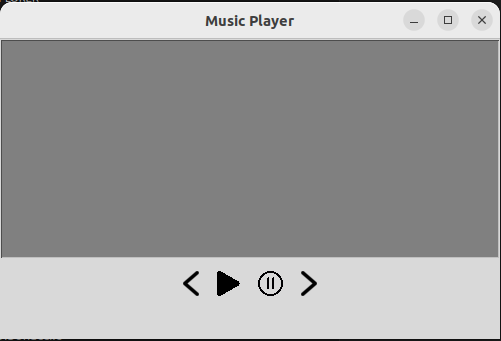
\includegraphics[scale = 0.5]{images/User_Interface_image.png}
        \caption{User Interface image}
        \label{fig:1}
\end{figure}

\section{Design and Implementation}
The project was divided into the following steps:
\begin{itemize}
\item Importing the required libraries: The tkinter library was imported for GUI creation, and the pygame library was imported for audio playback.

\item Loading music files: The project defined a function named load$\_$music() to load the music files from the "audioFiles" folder. Only MP3 files were considered, and the file names were stored in a list named songs.

\item Playing music: The function play$\_$music() was created to play the music. It loaded the selected song using pygame.mixer.music.load() and played it with pygame.mixer.music.play(). If the music was paused, the function resumed playback using pygame.mixer.music.unpause().

\item Pausing music: The pause$\_$music() function paused the currently playing music using pygame.mixer.music.pause().

\item Skipping to the next song: The next$\_$music() function was responsible for skipping to the next song. It incremented the count variable, which tracked the current song index, and loaded and played the corresponding song using pygame.mixer.music.load() and pygame.mixer.music.play(). If the end of the playlist was reached, the count was reset to 0, and the songs were shuffled again.

\item Returning to the previous song: The prev$\_$music() function allowed the user to go back to the previous song. It decremented the song$\_$count variable to track the history of played songs, loaded and played the previous song using pygame.mixer.music.load(), and resumed playback.

\item GUI creation: The project created a GUI window using tkinter with buttons for play, pause, next, and previous actions. Images were used for the button icons, and the corresponding functions were assigned to the button commands.
\end{itemize}

\section{Usage}
\begin{itemize}
\item Run the Python script containing the music player code.
\item The GUI window will appear.
\item Use the play, pause, next, and previous buttons to control the music playback.
\item The program will continue running until the GUI window is closed.
\end{itemize}

\section{Conclusion}
The Music Player project provides a basic music player application with features such as playing audio files and controlling playback. It demonstrates the use of Pygame and its audio capabilities in Python programming.





\end{document}
